%% First version paper for IEEE Radar 2015 Johannesburg
%% Version 0 by MR Inggs
%%   23/05/2015
%% Version 1.0 by MR Inggs responding to reviewer comments

%% bare_conf.tex
%% V1.3
%% 2007/01/11
%% by Michael Shell
%% See:
%% http://www.michaelshell.org/
%% for current contact information.
%%
%% This is a skeleton file demonstrating the use of IEEEtran.cls
%% (requires IEEEtran.cls version 1.7 or later) with an IEEE conference paper.
%%
%% Support sites:
%% http://www.michaelshell.org/tex/ieeetran/
%% http://www.ctan.org/tex-archive/macros/latex/contrib/IEEEtran/
%% and
%% http://www.ieee.org/

%%*************************************************************************
%% Legal Notice:
%% This code is offered as-is without any warranty either expressed or
%% implied; without even the implied warranty of MERCHANTABILITY or
%% FITNESS FOR A PARTICULAR PURPOSE! 
%% User assumes all risk.
%% In no event shall IEEE or any contributor to this code be liable for
%% any damages or losses, including, but not limited to, incidental,
%% consequential, or any other damages, resulting from the use or misuse
%% of any information contained here.
%%
%% All comments are the opinions of their respective authors and are not
%% necessarily endorsed by the IEEE.
%%
%% This work is distributed under the LaTeX Project Public License (LPPL)
%% ( http://www.latex-project.org/ ) version 1.3, and may be freely used,
%% distributed and modified. A copy of the LPPL, version 1.3, is included
%% in the base LaTeX documentation of all distributions of LaTeX released
%% 2003/12/01 or later.
%% Retain all contribution notices and credits.
%% ** Modified files should be clearly indicated as such, including  **
%% ** renaming them and changing author support contact information. **
%%
%% File list of work: IEEEtran.cls, IEEEtran_HOWTO.pdf, bare_adv.tex,
%%                    bare_conf.tex, bare_jrnl.tex, bare_jrnl_compsoc.tex
%%*************************************************************************

% *** Authors should verify (and, if needed, correct) their LaTeX system  ***
% *** with the testflow diagnostic prior to trusting their LaTeX platform ***
% *** with production work. IEEE's font choices can trigger bugs that do  ***
% *** not appear when using other class files.                            ***
% The testflow support page is at:
% http://www.michaelshell.org/tex/testflow/



% Note that the a4paper option is mainly intended so that authors in
% countries using A4 can easily print to A4 and see how their papers will
% look in print - the typesetting of the document will not typically be
% affected with changes in paper size (but the bottom and side margins will).
% Use the testflow package mentioned above to verify correct handling of
% both paper sizes by the user's LaTeX system.
%
% Also note that the "draftcls" or "draftclsnofoot", not "draft", option
% should be used if it is desired that the figures are to be displayed in
% draft mode.
%
\documentclass[conference]{IEEEtran}
% Add the compsoc option for Computer Society conferences.
%
% If IEEEtran.cls has not been installed into the LaTeX system files,
% manually specify the path to it like:
% \documentclass[conference]{../sty/IEEEtran}





% Some very useful LaTeX packages include:
% (uncomment the ones you want to load)


% *** MISC UTILITY PACKAGES ***
%
%\usepackage{ifpdf}
% Heiko Oberdiek's ifpdf.sty is very useful if you need conditional
% compilation based on whether the output is pdf or dvi.
% usage:
% \ifpdf
%   % pdf code
% \else
%   % dvi code
% \fi
% The latest version of ifpdf.sty can be obtained from:
% http://www.ctan.org/tex-archive/macros/latex/contrib/oberdiek/
% Also, note that IEEEtran.cls V1.7 and later provides a builtin
% \ifCLASSINFOpdf conditional that works the same way.
% When switching from latex to pdflatex and vice-versa, the compiler may
% have to be run twice to clear warning/error messages.






% *** CITATION PACKAGES ***
%
%\usepackage{cite}
% cite.sty was written by Donald Arseneau
% V1.6 and later of IEEEtran pre-defines the format of the cite.sty package
% \cite{} output to follow that of IEEE. Loading the cite package will
% result in citation numbers being automatically sorted and properly
% "compressed/ranged". e.g., [1], [9], [2], [7], [5], [6] without using
% cite.sty will become [1], [2], [5]--[7], [9] using cite.sty. cite.sty's
% \cite will automatically add leading space, if needed. Use cite.sty's
% noadjust option (cite.sty V3.8 and later) if you want to turn this off.
% cite.sty is already installed on most LaTeX systems. Be sure and use
% version 4.0 (2003-05-27) and later if using hyperref.sty. cite.sty does
% not currently provide for hyperlinked citations.
% The latest version can be obtained at:
% http://www.ctan.org/tex-archive/macros/latex/contrib/cite/
% The documentation is contained in the cite.sty file itself.






% *** GRAPHICS RELATED PACKAGES ***
%
\ifCLASSINFOpdf
  % \usepackage[pdftex]{graphicx}
  % declare the path(s) where your graphic files are
  % \graphicspath{{../pdf/}{../jpeg/}}
  % and their extensions so you won't have to specify these with
  % every instance of \includegraphics
  % \DeclareGraphicsExtensions{.pdf,.jpeg,.png}
\else
  % or other class option (dvipsone, dvipdf, if not using dvips). graphicx
  % will default to the driver specified in the system graphics.cfg if no
  % driver is specified.
  % \usepackage[dvips]{graphicx}
  % declare the path(s) where your graphic files are
  % \graphicspath{{../eps/}}
  % and their extensions so you won't have to specify these with
  % every instance of \includegraphics
  % \DeclareGraphicsExtensions{.eps}
\fi
% graphicx was written by David Carlisle and Sebastian Rahtz. It is
% required if you want graphics, photos, etc. graphicx.sty is already
% installed on most LaTeX systems. The latest version and documentation can
% be obtained at: 
% http://www.ctan.org/tex-archive/macros/latex/required/graphics/
% Another good source of documentation is "Using Imported Graphics in
% LaTeX2e" by Keith Reckdahl which can be found as epslatex.ps or
% epslatex.pdf at: http://www.ctan.org/tex-archive/info/
%
% latex, and pdflatex in dvi mode, support graphics in encapsulated
% postscript (.eps) format. pdflatex in pdf mode supports graphics
% in .pdf, .jpeg, .png and .mps (metapost) formats. Users should ensure
% that all non-photo figures use a vector format (.eps, .pdf, .mps) and
% not a bitmapped formats (.jpeg, .png). IEEE frowns on bitmapped formats
% which can result in "jaggedy"/blurry rendering of lines and letters as
% well as large increases in file sizes.
%
% You can find documentation about the pdfTeX application at:
% http://www.tug.org/applications/pdftex





% *** MATH PACKAGES ***
%
%\usepackage[cmex10]{amsmath}
% A popular package from the American Mathematical Society that provides
% many useful and powerful commands for dealing with mathematics. If using
% it, be sure to load this package with the cmex10 option to ensure that
% only type 1 fonts will utilized at all point sizes. Without this option,
% it is possible that some math symbols, particularly those within
% footnotes, will be rendered in bitmap form which will result in a
% document that can not be IEEE Xplore compliant!
%
% Also, note that the amsmath package sets \interdisplaylinepenalty to 10000
% thus preventing page breaks from occurring within multiline equations. Use:
%\interdisplaylinepenalty=2500
% after loading amsmath to restore such page breaks as IEEEtran.cls normally
% does. amsmath.sty is already installed on most LaTeX systems. The latest
% version and documentation can be obtained at:
% http://www.ctan.org/tex-archive/macros/latex/required/amslatex/math/





% *** SPECIALIZED LIST PACKAGES ***
%
%\usepackage{algorithmic}
% algorithmic.sty was written by Peter Williams and Rogerio Brito.
% This package provides an algorithmic environment fo describing algorithms.
% You can use the algorithmic environment in-text or within a figure
% environment to provide for a floating algorithm. Do NOT use the algorithm
% floating environment provided by algorithm.sty (by the same authors) or
% algorithm2e.sty (by Christophe Fiorio) as IEEE does not use dedicated
% algorithm float types and packages that provide these will not provide
% correct IEEE style captions. The latest version and documentation of
% algorithmic.sty can be obtained at:
% http://www.ctan.org/tex-archive/macros/latex/contrib/algorithms/
% There is also a support site at:
% http://algorithms.berlios.de/index.html
% Also of interest may be the (relatively newer and more customizable)
% algorithmicx.sty package by Szasz Janos:
% http://www.ctan.org/tex-archive/macros/latex/contrib/algorithmicx/




% *** ALIGNMENT PACKAGES ***
%
%\usepackage{array}
% Frank Mittelbach's and David Carlisle's array.sty patches and improves
% the standard LaTeX2e array and tabular environments to provide better
% appearance and additional user controls. As the default LaTeX2e table
% generation code is lacking to the point of almost being broken with
% respect to the quality of the end results, all users are strongly
% advised to use an enhanced (at the very least that provided by array.sty)
% set of table tools. array.sty is already installed on most systems. The
% latest version and documentation can be obtained at:
% http://www.ctan.org/tex-archive/macros/latex/required/tools/


%\usepackage{mdwmath}
%\usepackage{mdwtab}
% Also highly recommended is Mark Wooding's extremely powerful MDW tools,
% especially mdwmath.sty and mdwtab.sty which are used to format equations
% and tables, respectively. The MDWtools set is already installed on most
% LaTeX systems. The lastest version and documentation is available at:
% http://www.ctan.org/tex-archive/macros/latex/contrib/mdwtools/


% IEEEtran contains the IEEEeqnarray family of commands that can be used to
% generate multiline equations as well as matrices, tables, etc., of high
% quality.


%\usepackage{eqparbox}
% Also of notable interest is Scott Pakin's eqparbox package for creating
% (automatically sized) equal width boxes - aka "natural width parboxes".
% Available at:
% http://www.ctan.org/tex-archive/macros/latex/contrib/eqparbox/





% *** SUBFIGURE PACKAGES ***
%\usepackage[tight,footnotesize]{subfigure}
% subfigure.sty was written by Steven Douglas Cochran. This package makes it
% easy to put subfigures in your figures. e.g., "Figure 1a and 1b". For IEEE
% work, it is a good idea to load it with the tight package option to reduce
% the amount of white space around the subfigures. subfigure.sty is already
% installed on most LaTeX systems. The latest version and documentation can
% be obtained at:
% http://www.ctan.org/tex-archive/obsolete/macros/latex/contrib/subfigure/
% subfigure.sty has been superceeded by subfig.sty.



%\usepackage[caption=false]{caption}
%\usepackage[font=footnotesize]{subfig}
% subfig.sty, also written by Steven Douglas Cochran, is the modern
% replacement for subfigure.sty. However, subfig.sty requires and
% automatically loads Axel Sommerfeldt's caption.sty which will override
% IEEEtran.cls handling of captions and this will result in nonIEEE style
% figure/table captions. To prevent this problem, be sure and preload
% caption.sty with its "caption=false" package option. This is will preserve
% IEEEtran.cls handing of captions. Version 1.3 (2005/06/28) and later 
% (recommended due to many improvements over 1.2) of subfig.sty supports
% the caption=false option directly:
%\usepackage[caption=false,font=footnotesize]{subfig}
%
% The latest version and documentation can be obtained at:
% http://www.ctan.org/tex-archive/macros/latex/contrib/subfig/
% The latest version and documentation of caption.sty can be obtained at:
% http://www.ctan.org/tex-archive/macros/latex/contrib/caption/




% *** FLOAT PACKAGES ***
%
%\usepackage{fixltx2e}
% fixltx2e, the successor to the earlier fix2col.sty, was written by
% Frank Mittelbach and David Carlisle. This package corrects a few problems
% in the LaTeX2e kernel, the most notable of which is that in current
% LaTeX2e releases, the ordering of single and double column floats is not
% guaranteed to be preserved. Thus, an unpatched LaTeX2e can allow a
% single column figure to be placed prior to an earlier double column
% figure. The latest version and documentation can be found at:
% http://www.ctan.org/tex-archive/macros/latex/base/



%\usepackage{stfloats}
% stfloats.sty was written by Sigitas Tolusis. This package gives LaTeX2e
% the ability to do double column floats at the bottom of the page as well
% as the top. (e.g., "\begin{figure*}[!b]" is not normally possible in
% LaTeX2e). It also provides a command:
%\fnbelowfloat
% to enable the placement of footnotes below bottom floats (the standard
% LaTeX2e kernel puts them above bottom floats). This is an invasive package
% which rewrites many portions of the LaTeX2e float routines. It may not work
% with other packages that modify the LaTeX2e float routines. The latest
% version and documentation can be obtained at:
% http://www.ctan.org/tex-archive/macros/latex/contrib/sttools/
% Documentation is contained in the stfloats.sty comments as well as in the
% presfull.pdf file. Do not use the stfloats baselinefloat ability as IEEE
% does not allow \baselineskip to stretch. Authors submitting work to the
% IEEE should note that IEEE rarely uses double column equations and
% that authors should try to avoid such use. Do not be tempted to use the
% cuted.sty or midfloat.sty packages (also by Sigitas Tolusis) as IEEE does
% not format its papers in such ways.





% *** PDF, URL AND HYPERLINK PACKAGES ***
%
\usepackage{url}
% url.sty was written by Donald Arseneau. It provides better support for
% handling and breaking URLs. url.sty is already installed on most LaTeX
% systems. The latest version can be obtained at:
% http://www.ctan.org/tex-archive/macros/latex/contrib/misc/
% Read the url.sty source comments for usage information. Basically,
% \url{my_url_here}.





% *** Do not adjust lengths that control margins, column widths, etc. ***
% *** Do not use packages that alter fonts (such as pslatex).         ***
% There should be no need to do such things with IEEEtran.cls V1.6 and later.
% (Unless specifically asked to do so by the journal or conference you plan
% to submit to, of course. )


\usepackage[textsize=tiny]{todonotes}
\usepackage{amsmath}
\usepackage{amsfonts}
\usepackage{amssymb}
\usepackage{array}
\usepackage{subfigure}
\usepackage{ragged2e}
\usepackage{tabu}
\usepackage{balance}
% correct bad hyphenation here
\hyphenation{}


\begin{document}
%
% paper title
% can use linebreaks \\ within to get better formatting as desired
\title{NOISE JAMMING OF A FM BAND COMMENSAL RADAR}


% conference papers do not typically use \thanks and this command
% is locked out in conference mode. If really needed, such as for
% the acknowledgment of grants, issue a \IEEEoverridecommandlockouts
% after \documentclass

% for over three affiliations, or if they all won't fit within the width
% of the page, use this alternative format:
% 

\author{\IEEEauthorblockN{
Michael Inggs\IEEEauthorrefmark{1},
Craig Tong\IEEEauthorrefmark{1},
Daniel O'Hagan\IEEEauthorrefmark{1},
Urs B\"oniger\IEEEauthorrefmark{2}, 
Urs Siegenthaler\IEEEauthorrefmark{2},
Christof Sch\"upbach\IEEEauthorrefmark{2}, 
Hans Pratisto\IEEEauthorrefmark{2}
}

\IEEEauthorblockA{\IEEEauthorrefmark{1}Department of Electrical Engineering\\ Radar Remote Sensing Group (RRSG) \\
University of Cape Town,
Rondebosch, South Africa\\ michael.inggs@uct.ac.za}
\IEEEauthorblockA{\IEEEauthorrefmark{2}armasuisse, Thun, Switzerland
}}


% make the title area
\maketitle


% IEEEtran.cls defaults to using nonbold math in the Abstract.
% This preserves the distinction between vectors and scalars. However,
% if the conference you are submitting to favors bold math in the abstract,
% then you can use LaTeX's standard command \boldmath at the very start
% of the abstract to achieve this. Many IEEE journals/conferences frown on
% math in the abstract anyway.

% no keywords








\begin{abstract}
Commensal Radars (CRs) are a class of EM sensor that use the emissions of other systems to fulfill their function, without having any impact or collaboration with the emitter of opportunity. The jamming of Commensal Radar (CR) systems, and possible ECCM responses to such jamming have not received more than a passing reference in the open literature. We examine a specific case of an FM Band Commensal radar with a multi-receiver configuration (single transmit site, many spatially distributed receivers) and find that although modest jammer power can be very effective in jamming the CR, the unknown geometry and frequencies of operation of the Commensal Radar (CR) will make it difficult to jam in practice. Simple null steering by the CR receivers is very effective. We also note that the CR system requires excellent Electronic Support Measures (ESM) to be aware of electronic attack. The paper reviews the tactical situation, and the very sparse literature. This is followed by some analysis of the effect of noise jamming, followed by simulations of jamming, with and without receiver null steering, as well as some self-protection jamming.
\end{abstract}

% For peer review papers, you can put extra information on the cover
% page as needed:
% \ifCLASSOPTIONpeerreview
% \begin{center} \bfseries EDICS Category: 3-BBND \end{center}
% \fi
%
% For peerreview papers, this IEEEtran command inserts a page break and
% creates the second title. It will be ignored for other modes.
\IEEEpeerreviewmaketitle


%========================
\section{Introduction}
A Commensal Radar (CR)  has many forms, but requires a transmitter of opportunity to sense targets. It has no effect on the selected transmitter, and does not collaborate with it in any way. The architecture depends on how the system detects and tracks targets of interest. We thus have many examples called ``Passive Bistatic Radar'' (PBR), ``Passive Coherent Location``(PCL), and so on~\cite{willis:07, baugh:03}. In addition, since there are a multitude of broadcast and communications systems (including other, active, radars) there are many options. To keep our analysis simple, we focus on a CR  that uses a single transmit site combined with a multitude of spatially distributed receivers, thus fitting into the description, ``Passive Multistatic Radar'' (PMR)~\cite[Chapter 6]{willis:07}. However, we consider the effects of ECM on just one node of such a radar, together with its transmitter of opportunity, forming a PBR.

It is clear that CR is transitioning from a research topic to a serious contender as a sensor for civilian (Air Traffic Management)(ATM) and military applications. The latter use implies that it will be subject to Electronic Countermeasures (ECM), but this would also be in the former case for terrorist attacks on a country's ATM infrastructure, for example, or, inadvertent interference. We have carried out an extensive survey of the open literature, and did not find significant discussion of this topic. In fact, there is an optimistic view taken by the researchers in the field i.e. that CR will be robust against ECM~\cite{villano:13}. This view must be treated with caution, as the CR systems must consider ECM and appropriate Counter-ECM (ECCM) measures to reduce the effect of ECM.

We have also investigated the possible Counter-countermeasures (ECCM) that a CR might deploy when an attack occurs. We note that the CR must be supported by excellent Electronic Support Measures (ESM) to assist it in the task of determining that an attack has occurred, and what countermeasures are required.

We begin the paper with a review of the sparse literature,  a brief overview of the geometry and signal processing of a CR, especially the system that we shall investigate in depth. This is followed by calculations of the expected performance of an ECM system (specifically a noise jammer), with noise jamming simulation results.

The paper concludes with a brief discussion of ECCM that can be deployed, with an example in simulation.


%========================
\section{Literature Review}
The number of CR-related publications has grown substantially in recent years,
particularly in relations to algorithmic refinement. RadarConf 2015 in Arlington had
a track dedicated to CR for the duration of the conference. However, despite
the intensity of CR research throughout the world, there are very few publications
in the open literature that focus on ECM applied to CR.

Scholarly searches yield hits that mention various research
programmes and suggestions for ECM against CR, however, there is little
of technical rigour requiring review.

The NATO Advanced Modelling and Systems Applications for Passive Sensors group SET-164 has produced a comprehensive report on CR performance, particularly with regards to the impacts of clutter. Another NATO group, SCI-190 Electronic Countermeasures to Radar with High-Resolution and Extended Coherent Processing, has performed a small study of countermeasure against CR (SCI-190 was not exclusively focused on ECM against CR).

One of the main limiting aspects of jamming and deceiving CR is that
the receiver location is unknown.

In ~\cite{ohagan_irs} O'Hagan et al discuss an Active Fallback Component (AFC) that could be used along with CR with the intention of sustaining covert radar surveillance even in the event of broadcast infrastructure destruction. The AFC was discussed in terms of employing low-power, low probability of intercept, waveforms. The work was fundamentally a means of making CR robust and functional, even if their primary illumination source was disabled.   


%=======================
\section{Calculations of Jammer Effectiveness}

Willis' book contains a comprehensive set of calculations of the effectiveness of noise jamming on a bistatic radar~\cite[Chapter 6, section 6.7]{willis:07}. We will not repeat the results here. The approach taken is to consider the noise present in the bistatic receiver as an increase in receiver noise temperature. The coverage of a bistatic radar without directional antennas is predicted with closed form solutions, and the area covered by a system with ``benchmark range'' ($\sqrt{R_1 R_2}$ can be calculated. $R_1, R_2$ are the transmitter to target and target to receiver ranges where the signal to noise ratio is considered adequate for detection.

The presence of jammer noise reduces the SNR and hence, ``benchmark range'', and also, coverage area. The ratio of area with and without jamming is a measure of effectiveness of the jamming. The calculations presented in the reference~\cite[Chapter 6, section 6.7]{willis:07} show the sharp reduction in performance due to jamming. The approach does not take into account antenna directionality, and the non-linear processing of a real system. We decided to use simulation (FERS~\cite{inggs:09a, Brooker:2008c} ) to investigate a number of scenarios. FERS is a powerful simulator allowing for an arbitrary number of transmitters, targets and receivers to be assessed in complex scenarios.

%=======================
\section{Simulation Results}
For simplicity, we analyse a CR in the form of a PBR in the FM Broadcast Band (88 to 108~MHz). The geometry is given in Figure~\ref{fig:SimGeometryGE}. The parameters are typical of this type of system, of which the example is just one bistatic pair. To achieve tracking, a number of transmitters or receivers is required~\cite{maasdorp2014cramer}. The planning of such a system is also complex, to obtain optimum performance~\cite{inggs2014planning}.

%-----------------------------------------
\subsection{Simulation overview}

Referring to the figure, a receiver is located at the North most region of map labelled Malmesbury Rx. This receiver exploits an FM band transmitter labelled Constantiaberg Tx in the South West corner of the map. A jammer is positioned at a well known high site overlooking the entire region. This is located in the middle of the map. An aircraft flies from the North East which mimics the typical Johannesburg / Cape Town flight path of this region. The aircraft heads towards the Cape Town International Airport, labelled as CPT Airport. The simulation runs for 3 minutes during which time, the aircraft descends from 10000 to 5000~m, travel at a constant straight line velocity of 200~m/s. 

\begin{figure}[htbp]
\begin{center}
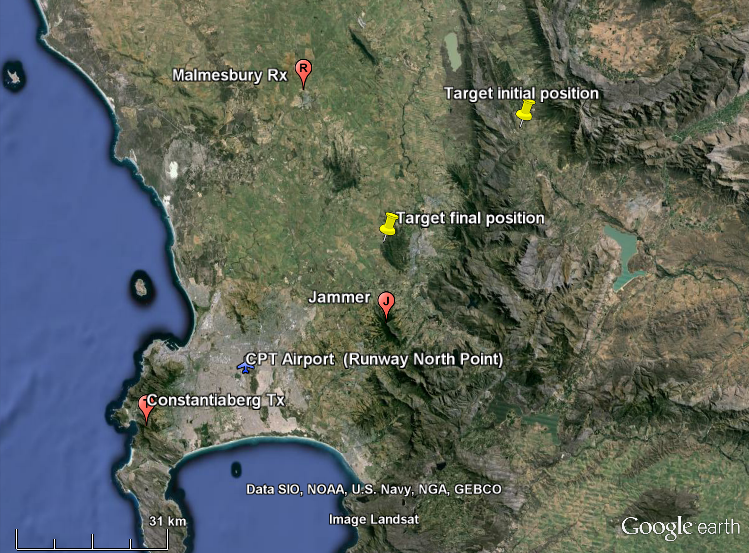
\includegraphics[width=0.9\columnwidth]{figs/Simulations/GEGeometryOverview.png}
\caption{An overview of the geometry for jamming simulations. North is upwards. The lateral scale in approximately 120~km by 100~km north-south.}
\label{fig:SimGeometryGE}
\end{center}
\end{figure}

The Constantiaberg transmitter radiates isotropically for simplicity. The radar receiver has a pair of 60 degree beam-width, 7.2 dBi antennas with a sinc function based response as shown in Figure~\ref{fig:AntennaBeam} for both vertical and horizontal planes. This is very similar to the Yagi antennas used in the prototype FM band radar at UCT~\cite{tong:14}. At the receiver site, the reference antenna points towards the Contastantiaberg transmitter. The surveillance antenna points towards the centre of the target flight path, i.e. between the 2 thumbtacks. The jammer has the same 7.2 dBi antenna as the receiver and points directly towards the receiver. Further details are given in Table~\ref{tab:SimulationParameters}.

\begin{figure}[htbp]
\begin{center}
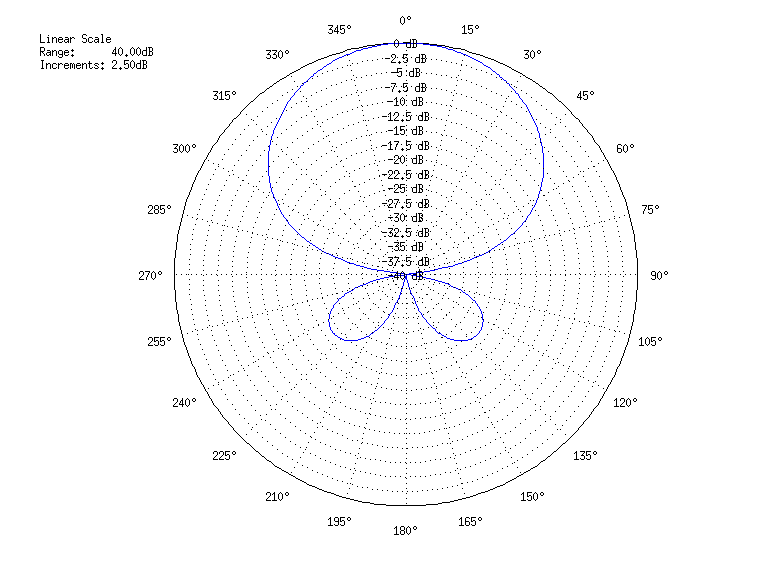
\includegraphics[width=0.9\columnwidth]{figs/Simulations/AntennaBeam.png}
\caption[Antenna pattern used in jamming simulations.]{Antenna beam used for the radar receiver and jammer. This pattern applies to both the horizontal and vertical. 0 dB boresight is equivalent to 7.2~dBi gain.}
\label{fig:AntennaBeam}
\end{center}
\end{figure}

\begin{table}[ht!]\label{tab:SimulationParameters}
\caption{Noise jammer simulation parameters.}

	\centering
	
	\vspace{1cm}
	\begin{tabu} to \columnwidth { X r }
  		Item 								& Parameter\\
  		\hline
  		\textbf{Transmitter} 				& \\
  		Antenna beam pattern 				& Isotropic\\
  		Antenna gain 						& 0 dB\\
  		Antenna altitude 					& 400~m\\
  		Power 								& 16.4~kW (EIRP for 10~kW dipole)\\
  		Carrier frequency					& 89~MHz\\
  		Waveform							& Real recorded FM data 204.8 kSps complex sampled\\[3mm]
  		
  		\textbf{Receiver} 					& \\
  		Antenna beam pattern 				& Sinc\\
  		Antenna gain 						& 7.2 dBi (see Figure~\ref{fig:AntennaBeam})\\
  		Antenna altitude					& 240~m\\
  		LO error							& ~50 ppb (std. dev. of 0.01~Hz @ 204.8 kSps)\\
  		Noise figure						& 4 dB\\
  		Digitisation						& 204.8 kSps complex, 16 bit quantisation\\[3mm]

		\textbf{Target} 					& \\
		Initial altitude					& 10000~m\\
		Final altitude						& 5000~m\\
		Velocity							& Constant 200~m/s\\
		RCS @ 89~MHz						& 46 dBsqm (200~m$^2$, a large airliner)\\[3mm]
		
		\textbf{Jammer} 					& \\
		Antenna beam pattern				& Sinc\\
  		Antenna gain 						& 7.2 dBi (see Figure~\ref{fig:AntennaBeam})\\
  		Transmit power						& 1, 5 and 10~W before antenna gain\\
  		Carrier frequency					& 89 MHz\\
  		Waveform							& 204.8 kSps complex, random noise\\[3mm]
  		
  		\textbf{Radar Signal Processing}	& \\
  		DPI cancellation					& 5 range, 5 Doppler bins\\
  		DPI cancellation CPI				& 102400 samples (0.5~s)\\
  		Range/Doppler processing			& 120 range, 1601 Doppler bins\\
  		Range/Doppler CPI					& 819200 samples (4~s)\\
  		CFAR algorithm						& GOCA-CFAR\\
  		CFAR window							& 4 guards, 8 reference cells (per side of CUT)\\
  		CFAR dimension						& Doppler (robust against bandwidth fluctuations)\\
  		CFAR threshold					    & P$_{fa}$ = 10$^{-5}$ (exponential noise model)\\
				  
	\end{tabu}
	
	\vspace{1cm}
	
\end{table}

\subsection{Illuminating Signal of Opportunity}

The illuminating signal of opportunity used in the simulation is real FM data recorded at the actual site on which the simulation is based. This site has a favourable interference environment and is relatively free of multipath. The data is stored as a complex baseband stream of IQ data sampled at 204.8 kSps. It is fed into the simulator in this form. The simulator software mixes the baseband data up to a carrier frequency of interest. This way the simulation will produce realistic bandwidth functions in the FM band signal as well as a realistic FM signal ambiguity function. The spectrum  of the FM signal is shown in Figure~\ref{fig:FMFrequencyResponse}.

\begin{figure}[htbp]
\begin{center}
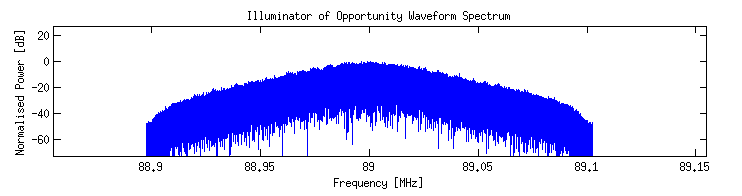
\includegraphics[width=0.9\columnwidth]{figs/Simulations/FMSpectrum.png}
\caption{The spectrum of the illuminator of opportunity (FM) signal shown at its RF frequency.}
\label{fig:FMFrequencyResponse}
\end{center}
\end{figure}

The equation for processing gain as shown in Equation~\ref{equ:ProcessingGain}, a maximum modulation bandwidth of 204.8 kHz in the 204.8 kSps complex data block would allow for an integration gain of around 60~dB assuming a 4 second integration time, as is consistent with such an FM band radar.

\begin{align}\label{equ:ProcessingGain}
G_{int} & = t_{int}  \beta\\
	    & = 10 \log{\bigg(4~s  \times 204.8~\mathrm{kHz}\bigg)}\\
	    & = 59.13~\mathrm{dB} ,
\end{align}

where $G_{int}$ is integration gain, $t_{int}$ is the integration time and $\beta$ is the bandwidth of the signal.

Also related to the modulation bandwidth is the range resolution: this relation is governed by Equation~\ref{equ:BistaticRangeRes}. In the case of the simulation which uses a 204.8~kSps (complex) signal and a carrier frequency of 89~MHz, the bin resolutions will be 1463.83~m and 0.25~Hz for bistatic range and bistatic Doppler resolutions respectively. 0.25~Hz is equivalent to 0.84~m/s bistatic range rate at 89~MHz.

\begin{equation}\label{equ:BistaticRangeRes}
\Delta R = \frac{c}{\beta \cos{  (\theta / 2 )}} ,
\end{equation}

where $\Delta R$ is the attainable bistatic range resolution in metres (which applies to the same dimension as bistatic range), $c$ is the speed of light in metres per second, $\beta$ is the instantaneous modulation bandwidth of the signal that is being exploited in Hertz and $\theta$ is the bistatic angle, that is, the angle formed by the transmitter-target and target-receiver line segments in radians. The minimum distance to which two separate targets can be distinguished will therefore be approximately twice that of the bistatic range resolution.


\subsection{Jamming Signal}

The jamming signal is generated as a complex 204.8 kSps random sequence, which, as such occupies the full bandwidth of the target FM channel.  The flat frequency response is characteristic of the noise like time domain signal, occupying 204.8 kHz of bandwidth. In practice the response of the RF frontend would attenuate the edge of the frequency pedestal.

The auto ambiguity function function of the jammer signal, which is the cross-ambiguity function of the jamming signal with itself, is a ``thumbtack'' response which can be attributed to the critically sampled noise signal that the jammer emits. 

A passive radar receiver receiving such a jamming signal on both its surveillance and reference channel would therefore suffer integrated interference across its range/Doppler plane. The peak level would be scaled according to the received signal strength at the receiver input.

\subsection{Simulation Runs}\label{sec:ECMSims}


The following runs are performed with the FERS simulator to gauge the effect of the jammer on the radar. The important plots that we show are the Amplitude Range Doppler (ARD) and Constant False Alarm Rate (CFAR). The former is, after clutter cancellation, bistatic range from left to right, and measured doppler shift vertically, with colour indicating the strength of the return after processing. The latter is the same plot, except that an area based filter is moved over the data to average out false signals, essentially converting the plot to two values target or no target. A number of CFAR plots are then overlaid, and signals that exceed the threshold are repeated, thereby showing a history of targets that exceed the threshold. For all the simulations presented here, the signal level of the plot has been normalised to the level of the target at the beginning of the first clean simulation run as shown in Figure~\ref{fig:NoJammingARDFirst} of the simulation without jamming. This way the noise and interference floor level can be compared directly to the signal level of the target return.

\subsubsection{No Jamming}
To establish a performance baseline a simulation with the target flying its specified trajectory with no interfering signal present.

The target displays a signal to noise ratio in the range of 25~to~30~dB for the duration of manoeuvre. This is consistent with actual measurements taken at the site exploiting the same transmitter and observing large commercial airliners flying along a similar trajectory. Figure~\ref{fig:NoJammingARDFirst} shows the range/Doppler map at the beginning of the target manoeuvre, Figure~\ref{fig:NoJammingARDLast} shows the range/Doppler map at the end of the target manoeuvre and Figure~\ref{fig:NoJammingARDCFAR} shows the CFAR filter detection history for all frames of the target manoeuvre.

\begin{figure}[htbp]
\begin{center}
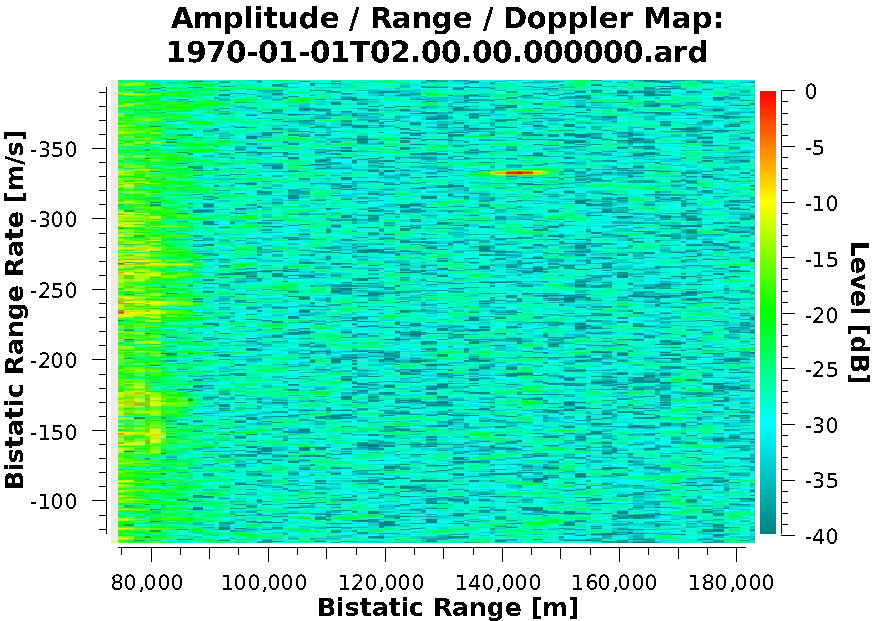
\includegraphics[width=1.0\columnwidth]{figs/Simulations/NoJammingARDFirst.pdf}
\caption{ARD at the beginning of the flight trajectory when no jamming is present.}
\label{fig:NoJammingARDFirst}
\end{center}
\end{figure}

\begin{figure}[htbp]
\begin{center}
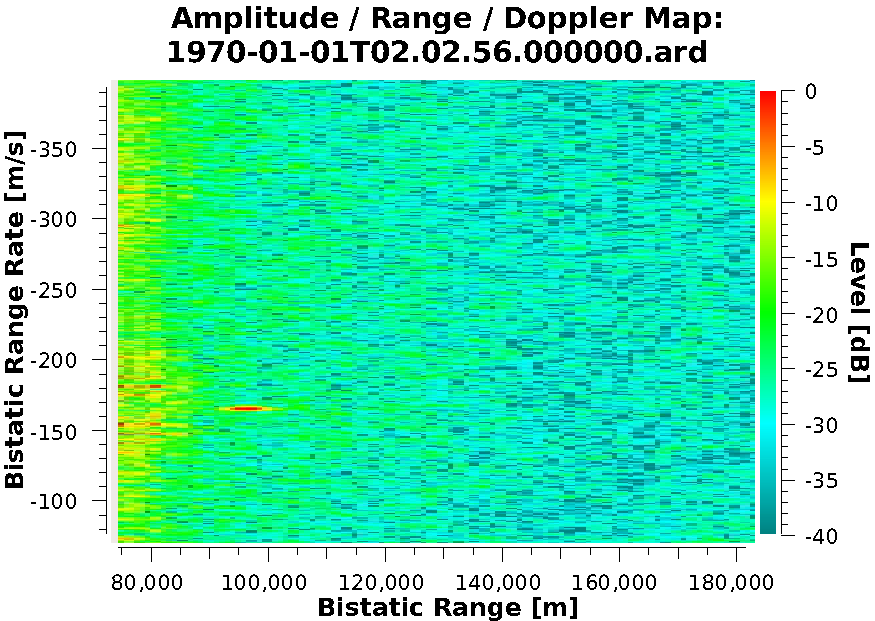
\includegraphics[width=01.0\columnwidth]{figs/Simulations/NoJammingARDLast.pdf}
\caption{ARD at the end of the flight trajectory when no jamming is present.}
\label{fig:NoJammingARDLast}
\end{center}
\end{figure}

We have included the signal and some of the data processing in our simulations, and Figure~\ref{fig:NoJammingARDCFAR} thus represents to plot extraction level, the output of a realistic CR. The analysis based only on SNR reduction~\cite[Chapter 6, section 6.7]{willis:07} does not include the highly non-linear effect of the clutter reduction and CFAR processing~\cite{tong:14}

\begin{figure}[htbp]
\begin{center}
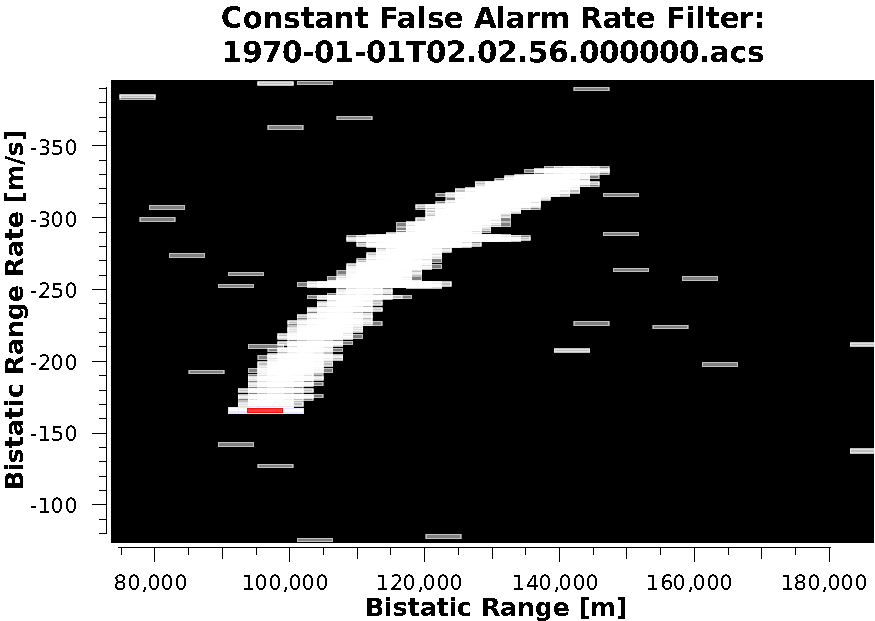
\includegraphics[width=1.0\columnwidth]{figs/Simulations/NoJammingCFAR.pdf}
\caption{CFAR history for the duration of the flight trajectory when no jamming is present.}
\label{fig:NoJammingARDCFAR}
\end{center}
\end{figure}

%\clearpage

\subsubsection{1W Jamming}

The jammer is now activated (see Figure~\ref{fig:SimGeometryGE}) with 1W of power feeding into the 7.2 dBi antenna which is directed at the radar receiver site. There is a noticeable rise in the noise floor and accordingly a drop in SINR, of approximately 10~dB. The CFAR filter is still able to detect the target through the manoeuvre. Figure~\ref{fig:1WJammingARDFirst} shows the range/Doppler map at the beginning of the target manoeuvre, and Figure~\ref{fig:1WJammingARDCFAR} shows the CFAR filter detection history for all frames of the target manoeuvre.

\begin{figure}[htbp]
\begin{center}
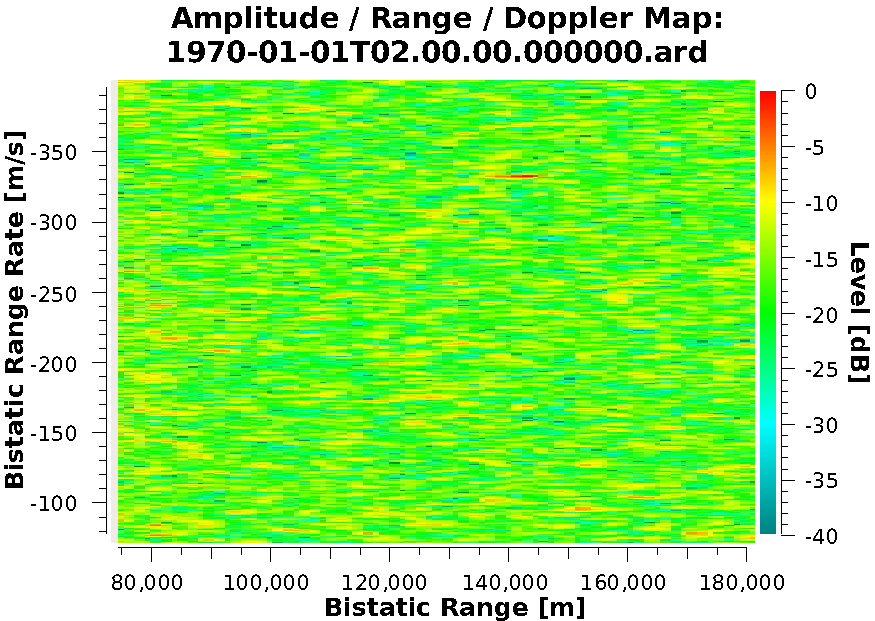
\includegraphics[width=1.0\columnwidth]{figs/Simulations/1WJammingARDFirst.pdf}
\caption{ARD at the beginning of the flight trajectory when 1~W jamming is present.}
\label{fig:1WJammingARDFirst}
\end{center}
\end{figure}



\begin{figure}[htbp]
\begin{center}
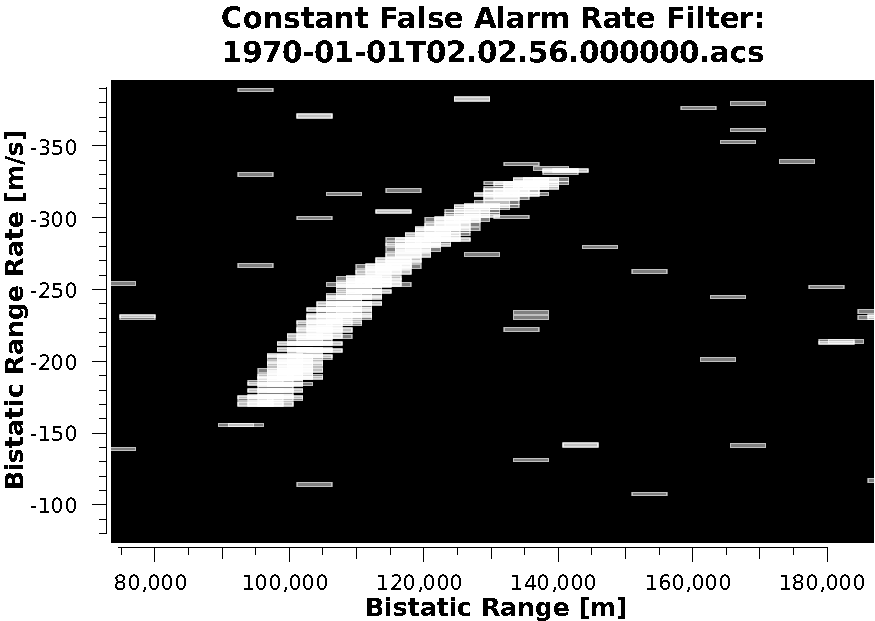
\includegraphics[width=1.0\columnwidth]{figs/Simulations/1WJammingCFAR.pdf}
\caption{CFAR history for the duration of the flight trajectory when 1~W jamming is present.}
\label{fig:1WJammingARDCFAR}
\end{center}
\end{figure}



\subsubsection{10W Jamming}\label{sec:Jam10W}

The noise jammer power is then increased to 10W. The target is no longer discernible in a single stationary ARD map. The interference floor is raised. The CFAR detector begins to loose a significant number of detections during the target manoeuvre. Figure~\ref{fig:10WJammingCFAR} shows the CFAR filter detection history for all frames of the target manoeuvre.


\begin{figure}[htbp]
\begin{center}
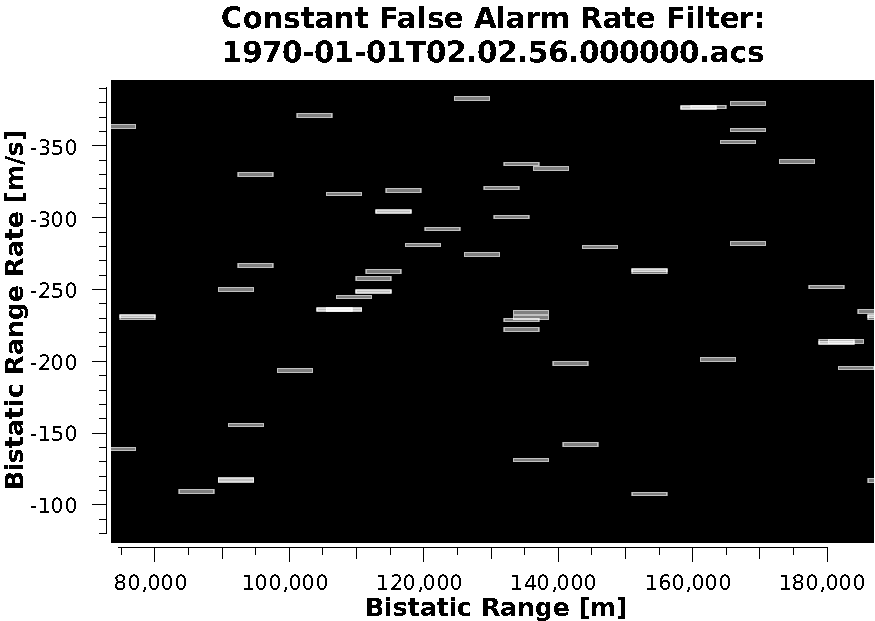
\includegraphics[width=1.0\columnwidth]{figs/Simulations/10WJammingCFAR.pdf}
\caption{CFAR history for the duration of the flight trajectory when 10~W jamming is present.}
\label{fig:10WJammingCFAR}
\end{center}
\end{figure}


\subsubsection{Target Self-protection}\label{sec:SelfProtection}

This section discussed the implications of the target radiating its own jamming signal. This is simulated with an omni-directional beam pattern. Only 1W of power is radiated given that airborne ECM platforms are likely to have power limitations. In effect the emitted signal is orders of magnitude larger than the target echo even at only 1~W and so masks the radar return effectively. Figure~\ref{fig:1WSelfProtectionCFAR} shows the CFAR trail for the entire trajectory. The target trajectory is not identifiable in the output map.


\begin{figure}[htbp]
\begin{center}
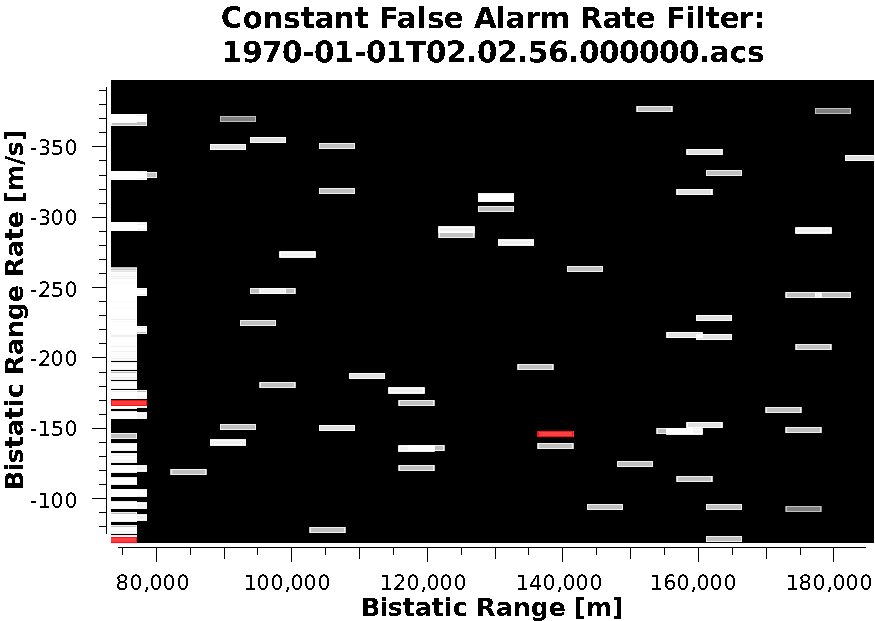
\includegraphics[width=1.0\columnwidth]{figs/Simulations/1WSelfProtectionCFAR.pdf}
\caption[CFAR 1~W self-protection jamming from the target. ]{CFAR history for the duration of the flight trajectory when 1~W self-protection jamming from the target is present.}
\label{fig:1WSelfProtectionCFAR}
\end{center}
\end{figure}

To investigate the effect of the self protection jamming further,  the ARD map shown at the beginning of the trajectory as in Figure~\ref{fig:1WSelfProtectionARDFirst_targetNormalised}, normalised to the level of the target return. The target return level is again derived as the jamming free interference simulation run as shown in Figure~\ref{fig:NoJammingARDFirst}. The normalised version  is shown in Figure~\ref{fig:1WSelfProtectionARDFirst_targetNormalised}. As can be observed the noise-plus-interference floor now sits some 20~dB above the level of the target so detection is highly unlikely.

\begin{figure}[htbp]
\begin{center}
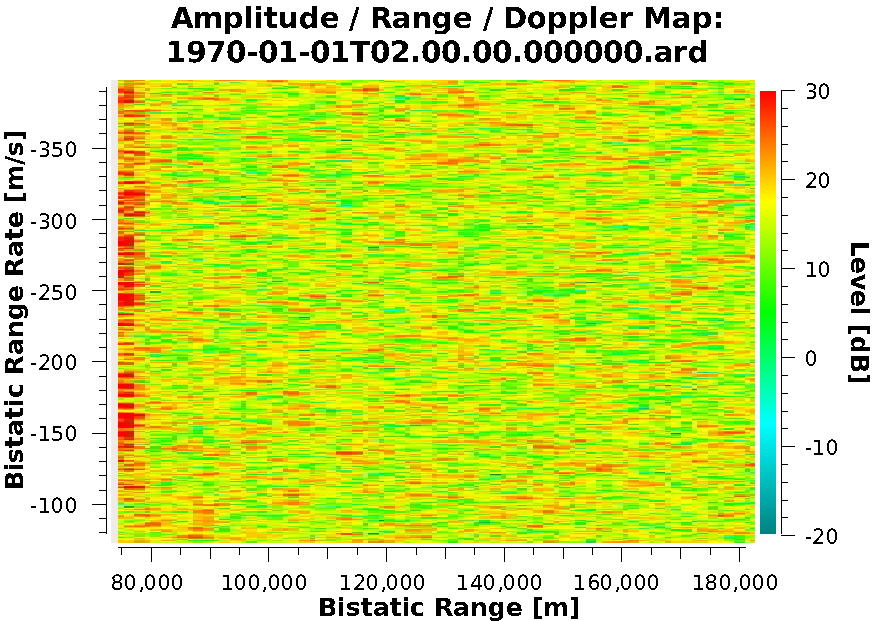
\includegraphics[width=1.0\columnwidth]{figs/Simulations/1WSelfProtectionARDFirstTargetNormalised.pdf}
\caption[ARD map normalised to target return.]{ARD at the beginning of the flight trajectory when 1~W self-protection jamming from the target is present. The map is normalised to the level of the target return.}
\label{fig:1WSelfProtectionARDFirst_targetNormalised}
\end{center}
\end{figure}

%========================
\subsection{ECCM}

Depending on the type of CR system, it should be possible to have an array type antenna, and then to have such an antenna steer a null toward the jamming source (assuming such a source's position or bearing is known). As shown in Willis~\cite{willis:07}, substantial improvement to CR system performance is possible, at the expense of having a \emph{wedge} taken out of the coverage by the surveillance channel null. A conventional ESM with AoA capability would be very useful to find the bearing and presence of a jamming source.

This is illustrated by simulation. Figure~\ref{fig:10WJammingNullSteeringCFAR} show the CFAR results repeating the 10~W jammer scenario described in Section~\ref{sec:Jam10W}. All details are the same except that the surveillance antenna is rotated to the North such that a 7.5 dB null (relative to the 7.2 dBi main lobe) is steered towards the jammer. It is shown that this gives suitable isolation to allow for target detection. Again the plots have been normalised to the target level which is now slightly lower due the main beam of the surveillance antenna not being centred on the target for the duration of its flight path. While the target is not present in the initial ARD map, it soon becomes detectable as can be seen by the CFAR history in Figure~\ref{fig:10WJammingNullSteeringCFAR}. 



\begin{figure}[htbp]
\begin{center}
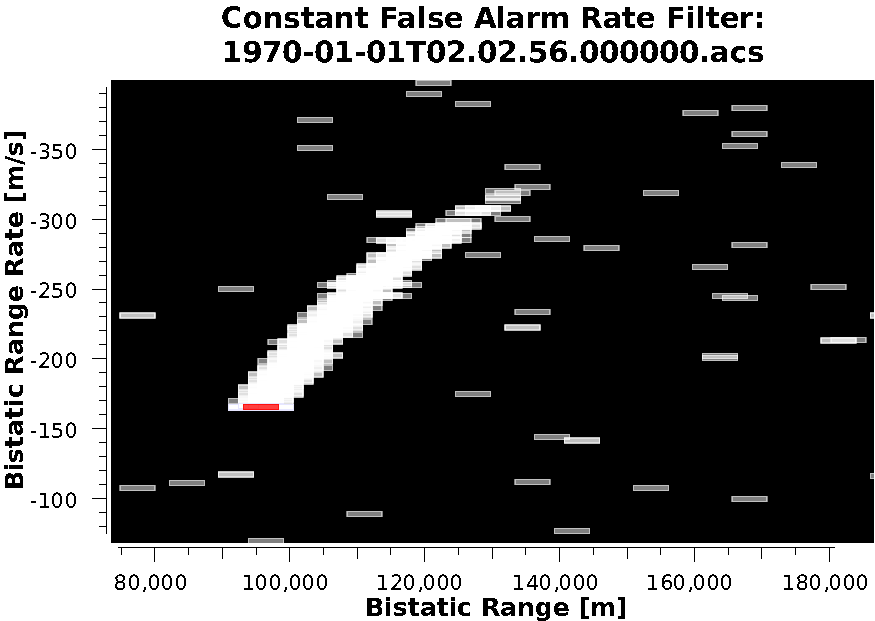
\includegraphics[width=1.0\columnwidth]{figs/Simulations/10WJammingNullSteeringCFAR.pdf}
\caption[CFAR history with null steered to jammer of 10~W.]{CFAR history for the duration of the flight trajectory when 10~W jamming present and a 7.5 dB null relative to bore-site gain is steered towards the jamming.}
\label{fig:10WJammingNullSteeringCFAR}
\end{center}
\end{figure}

\balance

CR systems that rely on a single receive station, and multiple transmitters will suffer most in terms of loss of angle coverage in utilising this sort of ECCM. However, a CR that uses multiple receive stations, spatially distributed, will have much more flexibility. This is somewhat difficult to quantify, as it is so specific to the actual installation of the CR. Arguing loosely, the wedge taken out from each system will point in a different direction for each receiver, leaving the aggregate performance of the system good. 
%--------------------------------------------------
\subsection{The Importance of ESM}

The presence of a noise jammer has an insidious effect on system performance, and it is clear that a CR system must be fitted with an ESM that is able to detect the presence of the jamming, frequency, and relative direction, so that ECCM can be triggered.


%========================
\section{Conclusions}

This paper has explored the effectiveness of ECM deployed again a CR. We demonstrate with a number of simulations the effectiveness of ECM when the CR System's positions are known. The effectiveness of a self-protection jammer is also shown. The simulations include typical signal processing, up to the plot extraction stage.

It is also clear that unless the jammer has prior knowledge of both frequency of operation, and the site of the CR system, mounting an ECM attach will be very difficult.

We point out the importance that a CR system is supported by excellent ESM, so that the presence, and bearing, of jamming can be detected. This will allow the CR to deploy ECCM null steering. It follows that a system with spatially diverse receivers will be very difficult to jam, as not all antennas will be exposed to the jammer. Simple null steering is an effective countermeasure to standoff jamming. However, self protection jamming cannot be mitigated. However, a platform carrying a jammer is in effect carrying a beacon, and DoA and other techniques can be used to find the target.

\nopagebreak
%=========== Bibliography =====================
%\newpage \addcontentsline{toc}{chapter}{Bibliography} % \nocite{*}
\bibliographystyle{vancouver}
\bibliography{CommensalJamming,doh_bib_1}
%================================


\end{document}  